\chapter{Python Basics}

We do not want to provide a full python tutorial, but rather formulate a guide through main steps and a setup which is very flexible to work with python and machine learning for weather, climate and environment. 

Our goal is to enable our scientists and developers to use python and machine learning in a flexible, modular and portable way for their development, for science as well as for products and services of various types. On the basis of python in combination with large language models we will touch the full workflow for science, development, product design and deployment. 

\section{Install, Virtual Environment, Pip und Import}

\subsection{Install and Virtual Environment}
\label{sec:virtualenv}

Before running Python commands, ensure you have Python installed. It is very easy to have Python installed on your laptop by simply downloading it - this is often possible without administration rights. You will then need to set the path variable properly. On Linux, depending on the version installed by your system administrator, you may find the executable under \texttt{python}, \texttt{python3}, \texttt{python3.11} or \texttt{python3.12}. We recommend not working with versions earlier than Python 3.10 because you may run into compatibility issues; instead, make sure you have an up-to-date Python version installed. Test the installed version by:

\begin{codeonly}{Test Python Installation}
python --version 
\end{codeonly}
  
Python has become one of the most popular programming languages, largely because of its extensive ecosystem of packages and libraries. From data analysis and visualization to machine learning and web development, Python's modular design allows you to choose only the components you need.

%------------------------------------------------------------------------------
% Graph Figure
%------------------------------------------------------------------------------
\begin{center}
\begin{tikzpicture}[>=Stealth,
  every node/.style={
    draw, 
    rounded corners, 
    align=center, 
    fill=blue!1, 
    font=\sffamily, 
    inner sep=1mm,
    minimum width=2.5cm, 
    minimum height=1cm
  },
  arrow/.style={-{Stealth[scale=1.2]}, thick}
]
  \matrix (m) [matrix of nodes, row sep=1cm, column sep=1cm, nodes={fill=DWDblue!100,text=white}]{
    & scipy & & \\
    numpy & & pandas & seaborn \\
    & matplotlib & & \\
  };

	\coordinate (via) at ($(m-2-1)!0.7!(m-2-4) + (0,-1)$);

  \draw[arrow] (m-2-1) -- (m-1-2);
  \draw[arrow] (m-2-1) -- (m-3-2);
  \draw[arrow] (m-1-2) -- (m-2-3);
  \draw[arrow] (m-3-2) -- (m-2-3);
  \draw[arrow] (m-2-3) -- (m-2-4);
  \draw[arrow] (m-2-1) -- (via) -- (m-2-4);
	
	\tikzset{
  explanation/.style={
    draw=none,         % No boundary
		fill=none, 
    font=\sffamily\fontseries{ul}\small,  
    align=center       % Centered text
    }
  }
	\tikzset{
  heading/.style={
    draw=none,         % No boundary
		fill=none, 
    font=\sffamily,  
    align=center       % Centered text
    }
  }
\node[heading, above=0mm of m] {\textbf{Package Tree Example}}; % numpy

\node[explanation, above=2mm of m-2-1] {Numerics}; % numpy
\node[explanation, below=2mm of m-1-2] {Scientific \\Computing}; % scipy
\node[explanation, above=2mm of m-3-2] {Visualization}; % scipy
\node[explanation, above=2mm of m-2-3] {Data \\Management}; % pandas
\node[explanation, below=2mm of m-2-4] {Statistical \\Visualization}; % seaborn

\end{tikzpicture}
\end{center}

It is very important to learn to manage packages to build a robust and tailored development environment. Learning how to install, manage, and create packages not only gives you a deeper understanding of the available tools, but also grants you greater control over your projects.

Usually, it is very important for a particular Python environment to provide a complete list of the packages it needs, with their versions, in a consistent framework. This framework is provided by \b1{virtual environments}.

A virtual environment allows you to control your package installations. Below are example commands for both Windows and Linux:

\begin{codeonly}{Windows Command}
python -m venv myenv
myenv\Scripts\activate
\end{codeonly}

\begin{codeonly}{Linux Command}
python3 -m venv myenv
source myenv/bin/activate
\end{codeonly}

\subsection{Using \texttt{pip} to Manage Python Packages}

\noindent \texttt{pip} is the package installer for Python. It allows you to install, update, and manage packages from the Python Package Index (PyPI). For example, you can check the version of \texttt{pip}, list installed packages, and install popular packages like \texttt{numpy} and \texttt{matplotlib}. The following commands illustrate these basic operations:

\begin{codeonly}{Basic pip Commands}
pip --version
pip list
pip install numpy
pip install matplotlib
\end{codeonly}

\noindent These commands, when run in your command prompt or terminal, will display the current version of \texttt{pip}, show all installed Python packages, and install \texttt{numpy} and \texttt{matplotlib}, respectively.

One of the most widely used libraries in Python is \texttt{NumPy}, which provides powerful array objects and routines for fast numerical computation. 


%==============================================================================
%
%==============================================================================
\section{Managing Dependencies with \texttt{requirements.txt}}

Managing dependencies is crucial in Python projects, especially when working in different environments or collaborating with others. The \texttt{requirements.txt} file allows you to list all your project’s dependencies and their versions, making it easy to replicate the environment anywhere.

%==============================================================================
%
%==============================================================================
\subsubsection{Generating a \texttt{requirements.txt}}

If you already have a virtual environment set up and want to generate a \texttt{requirements.txt} file from it, first activate your current virtual environment. Once the virtual environment is activated, run the following command to generate the \texttt{requirements.txt} file:

\begin{codeonly}{Generate \texttt{requirements.txt}}
pip freeze > requirements.txt
\end{codeonly}

This creates a file named \texttt{requirements.txt} in your current working directory containing all installed packages and their versions, leading to e.g.\ the following simple requirements.txt file. 

\begin{codeonly}{Requirements.txt}
numpy==1.26.4
ollama==0.3.1
openai==1.69.0
openai-whisper==20240930
toml==0.10.2
torch==2.4.0
torch_geometric==2.5.3
torchmetrics==1.4.1
torchvision==0.19.0
\end{codeonly}

%==============================================================================
%
%==============================================================================
\subsubsection{Installing Dependencies from \texttt{requirements.txt}}

To install all dependencies from an existing \texttt{requirements.txt} file into a new virtual environment, first create and activate the environment as shown in Section~\ref{sec:virtualenv}. Then, run the following command:

\begin{codeonly}{Install Dependencies from \texttt{requirements.txt}}
pip install -r requirements.txt
\end{codeonly}

This installs all packages listed in the \texttt{requirements.txt} file, ensuring that your environment matches the specified dependencies.

With these steps, you can easily share and reproduce Python environments using \texttt{requirements.txt}.

%==============================================================================
%
%==============================================================================
\subsection{Importing Functions or Packages vs. Installation}

In Python, you can either directly import functions and modules from local files or install packages to make them globally available across projects. Understanding the difference is essential for maintaining clean and scalable code.

%==============================================================================
%
%==============================================================================
\subsubsection{Importing Functions or Packages}


You can import Python modules or functions directly from local \texttt{.py} files. For example, if you have the following structure:

\begin{lstlisting}[basicstyle=\ttfamily\small]
|
|-- main_greetings.py
|-- greetings.py
\end{lstlisting}

In \texttt{main\_greetings.py}, you can import from \texttt{greetings.py} as follows:

\begin{codeonly}{greetings.py}
# main.py
from greetings import say_hello

say_hello()
\end{codeonly}

This method is quick and easy for small projects but becomes difficult to manage as your codebase grows or when sharing across multiple projects. You should then create installable packages, we discuss in a moment. 

%==============================================================================
%
%==============================================================================
\subsubsection{The \texttt{importlib} Package in Python}

The \texttt{importlib} package allows you to reload Python modules without restarting the interpreter, which is especially useful during development when modifying code. Normally, Python imports a module only once per session, but \texttt{importlib.reload(module)} forces the interpreter to reload it, reflecting any recent changes. This is particularly handy in interactive environments like Jupyter Notebooks, where you want to see immediate updates after editing a module without restarting the entire session.

\begin{codeonly}{reload\_demo\_fkt.py}
# reload_demo_fkt.py

def greet(name):
    return f"Hello {name}"
\end{codeonly}

And now lets load it, then change the file and reload it. 

\begin{codeonly}{reload\_demo.py}
# reload_demo.py

import importlib
import reload_demo_fkt as mo

def replace_in_file(str1, str2, filename):
    with open(filename, 'r') as file:
        content = file.read()
    content = content.replace(str1, str2)
    with open(filename, 'w') as file:
        file.write(content)

# Call the greet function initially
print(mo.greet("Roland"))  # Expected: Hello Roland

# After modifying reload_demo_fkt.py, reload it
replace_in_file("Hello", "Good Morning", "reload_demo_fkt.py")

importlib.reload(mo)

# Call the updated greet function
print(mo.greet("Roland"))  # Expected: Good Morning Roland

# Restore the original version of the file
replace_in_file("Good Morning", "Hello", "reload_demo_fkt.py")
\end{codeonly}

%==============================================================================
%
%==============================================================================
\subsubsection{Creating an Installable Python Package}


An installable package allows you to reuse and share code easily across different environments. Consider the following structure:

\begin{lstlisting}[basicstyle=\ttfamily\small]
install_demo02/
|-- pyproject.toml
|-- README.md
+-- src/
    +-- install_demo02/
        |-- __init__.py
        |-- install_mod1.py
        |-- install_mod2.py

\end{lstlisting}

The project is defined in a \texttt{pyproject.toml} file, which can include a list of dependencies, that would replace the \texttt{requirements.txt}:

\begin{codeonly}{basic \texttt{pyproject.toml} file}
[build-system]
requires = [ "setuptools>=61"]
build-backend = "setuptools.build_meta"

[project]
name = "install_demo02"   # name of the directory in src/
version = "0.1.3"
description = "A simple Python package with greeting functions"
authors = [
  { name = "Roland Potthast", email = "Roland.Potthast@dwd.de" },
]
requires-python = ">=3.8"
#dependencies = ["numpy<2", "matplotlib",]

[tool.setuptools.packages.find]
where = ["src"]
\end{codeonly}

To install your package locally, in the \texttt{code} folder run:

\begin{codeonly}{Install Your Package}
pip install -e install_demo02/
\end{codeonly}

Once installed, you can import it in any project without reference to the location of the package, as in the file
\texttt{install\_demo\_test\_script.py}: 

\begin{codeonly}{install\_demo\_test\_script.py}
from install_demo02 import greet1, greet2

print(greet1("World"))  # Hello World!
print(greet2("World"))  # Good Morning World!
\end{codeonly}

\textbf{Legacy projects with \texttt{setup.py}}

Before \texttt{pyproject.toml} was invented, packages were defined in a \texttt{setup.py} file.
One can find an example package using \texttt{setup.py} in the \texttt{code/install\_demo} directory.

To make \texttt{setup.py} work on Windows, one might has to use the following steps.
\begin{lstlisting}{}
pip install setuptools wheel
pip install -e install_demo/ --no-build-isolation --no-use-pep517
\end{lstlisting}


%------------------------------------------------------------------------------
%
%------------------------------------------------------------------------------
\noindent \textbf{When to use each approach:}

\begin{itemize}
    \item \emph{Pure Import}: Use for small, single-project code or quick prototypes.
    \item \emph{Installable Package}: Use for larger projects, sharing code, and managing dependencies.
\end{itemize}

%==============================================================================
%
%==============================================================================
\subsubsection{Example: Installing from GitHub}


You can also install packages directly from Git repositories. For example:

\begin{codeonly}{Install from GitHub}
pip install git+https://github.com/username/my_package.git
\end{codeonly}

This installs your package from GitHub, making it easy to share code across teams and projects.

\subsection{What is PyPI?}

The Python Package Index (\textbf{PyPI}) is the official repository for third-party Python packages. It allows developers to:

\begin{itemize}
  \item Upload and share their Python projects with the community.
  \item Install packages using the \texttt{pip} tool.
  \item Manage versions and dependencies of published packages.
\end{itemize}

When a user runs \texttt{pip install some-package}, \texttt{pip} connects to PyPI to find and download the corresponding package.

To make a project available on PyPI, developers package their code (typically using \texttt{pyproject.toml} and tools like \texttt{setuptools} or \texttt{flit}), build the distribution, and upload it using \texttt{twine}.

Uploaded packages are then publicly available for installation and reuse.

For more information, visit the official website:

\href{https://pypi.org}{\texttt{https://pypi.org}}



%==============================================================================
%
%==============================================================================
\section{Introduction to NumPy}

NumPy is the fundamental package for numerical computing in Python. It provides the \texttt{ndarray}, a multidimensional array object that enables fast vectorized operations and efficient handling of large datasets. Although Python is known for its readability, NumPy’s power lies in its ability to perform operations on entire arrays without writing explicit loops—a major benefit for programmers experienced in other languages.

In NumPy, the core building block is the \texttt{ndarray}. An \texttt{ndarray} can be created from a Python list (or nested lists for multidimensional arrays), and it supports element-wise operations. This vectorized computation model is not only more concise but also significantly faster for large-scale computations. Consider the following example:

\begin{codeonly}{Creating Basic Arrays}
import numpy as np
arr1 = np.array([1, 2, 3, 4, 5])
print("1D array:", arr1)
arr2 = np.array([[1, 2, 3], [4, 5, 6]])
print("2D array:")
print(arr2)
\end{codeonly}

The code above shows how to import NumPy (commonly aliased as \texttt{np}) and create both one-dimensional and two-dimensional arrays. Instead of writing loops to process elements, you can use array operations that are both elegant and efficient.

%==============================================================================
%
%==============================================================================
\subsection{Vectorized Operations and Predefined Arrays}

One of NumPy’s most powerful features is vectorized operations. Instead of iterating over each element, you can perform operations on entire arrays with a single expression:

\begin{codeonly}{Vectorized Operations}
import numpy as np
a = np.array([1, 2, 3, 4, 5])
b = np.array([10, 20, 30, 40, 50])
c = a + b
d = a * b
print("Addition:", c)
print("Multiplication:", d)
\end{codeonly}

In addition to these operations, NumPy offers a variety of functions for creating arrays with predefined values. This is useful for initializing data or generating test datasets:

\begin{codeonly}{Predefined Arrays}
import numpy as np
zeros = np.zeros((3, 4))
print("Zeros array:")
print(zeros)
ones = np.ones((2, 5))
print("Ones array:")
print(ones)
range_array = np.arange(0, 10, 2)
print("Range array:", range_array)
linspace_array = np.linspace(0, 1, 5)
print("Linspace array:", linspace_array)
\end{codeonly}

%==============================================================================
%
%==============================================================================
\subsection{Slicing, Indexing, and Broadcasting}

NumPy arrays support powerful slicing and indexing methods, similar to Python lists but extended to multiple dimensions. This feature allows you to extract subarrays efficiently without copying the data:

\begin{codeonly}{Slicing and Indexing}
import numpy as np
matrix = np.array([[ 1,  2,  3,  4],
                   [ 5,  6,  7,  8],
                   [ 9, 10, 11, 12],
                   [13, 14, 15, 16]])
submatrix = matrix[1:4, 1:4]
print("Submatrix:")
print(submatrix)
element = matrix[1, 2]
print("Element at (2,3):", element)
\end{codeonly}

Broadcasting allows operations between arrays of different shapes. With broadcasting, NumPy automatically expands the dimensions of an array during arithmetic operations:

\begin{codeonly}{Broadcasting Example}
import numpy as np
mat = np.array([[1, 2, 3],
                [4, 5, 6],
                [7, 8, 9]])
vec = np.array([1, 0, -1])
result = mat - vec
print("Broadcasting result:")
print(result)
\end{codeonly}

%==============================================================================
%
%==============================================================================
\subsection{Mathematical Functions and Applications}

NumPy offers a comprehensive suite of mathematical functions that operate element-wise on arrays. Whether you need trigonometric, logarithmic, or exponential functions, NumPy has you covered:

\begin{codeonly}{Mathematical Functions}
import numpy as np
angles = np.linspace(0, np.pi, 5)
print("Angles:", angles)
sine_values = np.sin(angles)
print("Sine values:", sine_values)
exp_values = np.exp(np.array([0, 1, 2]))
print("Exponential values:", exp_values)
\end{codeonly}

Using these functions, you can perform complex numerical computations with minimal code. For example, you might model a physical phenomenon or simulate data; NumPy’s capabilities allow you to transform and analyze data efficiently Experiment with these examples, and explore further functionalities of NumPy to fully leverage Python's capabilities in scientific computing.

\begin{recommendationbox}
Make sure you know your basic python commands well! Initially, do not rely only on sophisticated packages. Keep the core python level as your active knowledge!
\end{recommendationbox}

%==============================================================================
%
%==============================================================================
\section{Generating Plots based on Matplotlib}

Paired with \texttt{Matplotlib}, a versatile plotting library, you can quickly visualize data and test your ideas. 

%==============================================================================
%
%==============================================================================
\subsection{1D Plots}
The following example demonstrates how to use these libraries to plot a simple curve. In this code snippet, we generate a sine wave using \texttt{NumPy} and then plot it with \texttt{Matplotlib}.

\begin{codeonly}{plot-sine-wave.py}
import numpy as np
import matplotlib.pyplot as plt

# Generate data
x = np.linspace(0, 10, 100)
y = np.sin(x)

# Create the plot
plt.figure(figsize=(4, 3))
plt.plot(x, y)
plt.xlabel('x')
plt.ylabel('sin(x)')
plt.title('Image generated by Simple Python Code')

# Save the plot as a PNG file
plt.savefig('images/plot-sine-wave.png')
plt.close()  # Close the figure to free up memory
\end{codeonly}

\begin{center}
   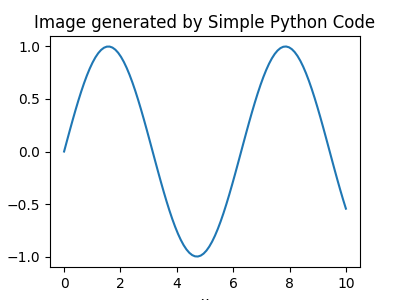
\includegraphics[width=0.6\textwidth]{images/plot-sine-wave.png}
\end{center}%

%==============================================================================
%
%==============================================================================
\subsection{2D Plots}

The following code demonstrates how to generate and visualize a two-dimensional field using NumPy and Matplotlib. First, a symmetric grid of x and y values is created and the radial distance from the origin is computed. Then, a Gaussian-modulated cosine function is used to define a smoothly varying field that decays with distance from the center. Finally, a filled contour plot is generated to visualize the field, and the resulting image is saved as a PNG file.

\begin{codeonly}{plot-gaussian-modulated-cosine-field.py}
import numpy as np
import matplotlib.pyplot as plt

# Create a grid of x and y values (centered at 0 for a symmetric field)
x = np.linspace(-10, 10, 200)
y = np.linspace(-10, 10, 200)
X, Y = np.meshgrid(x, y)

# Compute the radial distance from the origin
R = np.sqrt(X**2 + Y**2)

# Define a Gaussian-modulated cosine field
Z = np.exp(-0.1*(X**2 + Y**2)) * np.cos(5*R)

# Create a filled contour plot for the 2D field
plt.figure(figsize=(4, 3))
contour = plt.contourf(X, Y, Z, levels=50, cmap='viridis')
plt.colorbar(contour, label='Field value')
plt.xlabel('X')
plt.ylabel('Y')
plt.title('2D Field Plot: Gaussian-Modulated Cosine')
plt.savefig('images/plot-gaussian-modulated-cosine-field.png')
plt.close()
\end{codeonly}

\begin{center}
   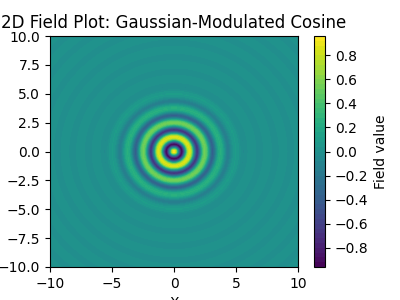
\includegraphics[width=0.6\textwidth]{images/plot-gaussian-modulated-cosine-field.png}
\end{center}%

The next example demonstrates how to create a simple 3D surface plot using Matplotlib's built-in \texttt{mplot3d} toolkit. By generating a meshgrid of \(x\) and \(y\) values and computing a corresponding \(z\) value from a radial sine function, the plot visualizes a three-dimensional wave-like pattern. This technique provides a straightforward way to represent and explore three-dimensional data in Python.

\begin{codeonly}{}

\end{codeonly}

\begin{center}
   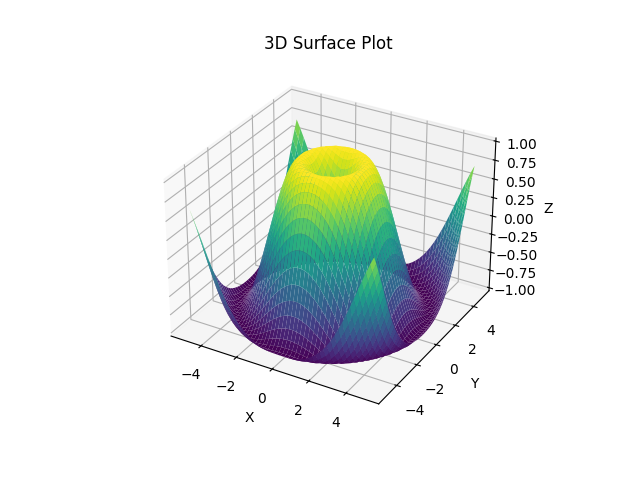
\includegraphics[width=0.6\textwidth]{images/plot-3d-surface.png}
\end{center}%

%==============================================================================
%
%==============================================================================
\section{Functions}

Python functions are reusable blocks of code that allow you to encapsulate logic and perform specific tasks. In Python, functions are defined using the \texttt{def} keyword and can take parameters, return values, and include documentation. The following sections introduce the basics of defining and using functions in Python.

%==============================================================================
%
%==============================================================================
\subsection{Defining a Function}
Functions are defined with the \texttt{def} keyword followed by the function name, parentheses containing any parameters, and a colon. The function body is indented. Here is a basic example that defines a function to greet a user:

\begin{codeonly}{Defining a Function}
def greet(name):
    """Return a greeting message."""
    return f"Hello, {name}!"
\end{codeonly}

%==============================================================================
%
%==============================================================================
\subsection{Calling a Function}
Once a function is defined, you can call it by using its name followed by parentheses containing any required arguments. The following example shows how to call the \texttt{greet} function and print its result:

\begin{codeonly}{Calling a Function}
message = greet("Alice")
print(message)
\end{codeonly}

%==============================================================================
%
%==============================================================================
\subsection{Functions with Multiple Parameters}
A function can accept multiple parameters. Below is an example of a function that calculates the area of a rectangle:

\begin{codeonly}{Function with Multiple Parameters}
def rectangle_area(width, height):
    """Calculate the area of a rectangle."""
    return width * height

area = rectangle_area(5, 3)
print("The area of the rectangle is:", area)
\end{codeonly}

%==============================================================================
%
%==============================================================================
\subsection{Default Parameter Values}
Python functions can have default parameter values, which are used when an argument is not provided. This example demonstrates a function that computes a power, using a default exponent of 2:

\begin{codeonly}{Default Parameter Values}
def power(number, exponent=2):
    """Return number raised to the power of exponent."""
    return number ** exponent

print(power(4))    # Uses default exponent 2 (result: 16)
print(power(2, 3)) # Exponent explicitly set to 3 (result: 8)
\end{codeonly}

%==============================================================================
%
%==============================================================================
\subsubsection{Variable-Length Arguments}
Sometimes, you may not know in advance how many arguments a function should accept. Python allows you to capture additional positional arguments using the \texttt{*args} syntax. In the following example, a function computes the sum of an arbitrary number of numbers:

\begin{codeonly}{Variable-Length Arguments}
def total_sum(*args):
    """Return the sum of all provided arguments."""
    return sum(args)

print(total_sum(1, 2, 3, 4, 5))  # Output: 15
\end{codeonly}


%==============================================================================
%
%==============================================================================
\section{Python Essentials}

Let us look at a survey table what basic python knowledge you should gain in a first step. 
We have already gone over some sigificant part of this, and will briefly give you a head-start for
the remaining points. 

\begin{table}[h!]
\centering
\begin{tabular}{|p{4cm}|p{8cm}|}
\hline
\textbf{Topic} & \textbf{Description} \\ \hline
Python Syntax & Basic structure, indentation, comments \\ \hline
Data Types & Integers, floats, strings, booleans, lists, tuples, sets, dictionaries \\ \hline
Control Flow & \texttt{if-else}, \texttt{for} and \texttt{while} loops, \texttt{break}, \texttt{continue} \\ \hline
Functions & Defining functions with \texttt{def}, arguments, return values, lambda functions \\ \hline
Modules and Imports & Importing built-in and external libraries, creating custom modules \\ \hline
File I/O & Reading and writing files, using \texttt{with} statements \\ \hline
Exception Handling & Using \texttt{try-except} for error handling \\ \hline
Object-Oriented Programming (OOP) & Classes, objects, inheritance, and polymorphism \\ \hline
Standard Libraries & Common libraries like \texttt{os}, \texttt{sys}, \texttt{math}, \texttt{datetime}, \texttt{json} \\ \hline
Virtual Environments & Creating and managing virtual environments with \texttt{venv} or \texttt{conda} \\ \hline
\end{tabular}
\caption{Essential Topics for Basic Python Learning}
\label{tab:basic_python_topics}
\end{table}

%==============================================================================
%
%==============================================================================
\subsection{Control Flow in Python}

Control flow in Python refers to the order in which individual statements, instructions, or function calls are executed. Python provides several structures for controlling the flow of your program, including conditionals, loops, and exception handling.

%==============================================================================
%
%==============================================================================
\subsubsection{Conditional Statements}

Conditional statements allow you to execute different code blocks based on certain conditions.

\textbf{Example:}
\begin{codeonly}{If-Else Statements}
x = 10
if x > 0:
    print("Positive")
elif x == 0:
    print("Zero")
else:
    print("Negative")
\end{codeonly}

%==============================================================================
%
%==============================================================================
\subsubsection{Loops}

Loops allow you to repeat a block of code multiple times.

\textbf{For Loop Example:}
\begin{codeonly}{For Loop}
for i in range(5):
    print(i)
\end{codeonly}

\textbf{While Loop Example:}
\begin{codeonly}{While Loop}
count = 0
while count < 5:
    print(count)
    count += 1
\end{codeonly}

%==============================================================================
%
%==============================================================================
\subsubsection{Loop Control Statements}

Python provides special statements to control the flow inside loops:
\begin{itemize}
    \item \texttt{break} – Exits the loop prematurely.
    \item \texttt{continue} – Skips the rest of the current iteration.
    \item \texttt{pass} – Does nothing and acts as a placeholder.
\end{itemize}

\textbf{Example with \texttt{break} and \texttt{continue}:}
\begin{codeonly}{Loop Control Example}
for i in range(10):
    if i == 3:
        continue  # Skip 3
    if i == 7:
        break  # Stop loop at 7
    print(i)
\end{codeonly}

%==============================================================================
%
%==============================================================================
\subsubsection{Exception Handling}

Python allows you to handle errors using \texttt{try-except} blocks to prevent program crashes.

\textbf{Example:}
\begin{codeonly}{Try-Except Block}
try:
    result = 10 / 0
except ZeroDivisionError:
    print("Cannot divide by zero!")
\end{codeonly}

\textbf{Summary:} Control flow structures are essential for building logical and efficient Python programs, allowing you to make decisions, iterate over data, and handle errors gracefully.


%==============================================================================
%
%==============================================================================
\subsection{File Input and Output in Python}

Python provides built-in functions to handle files, making it easy to read from and write to files. This section covers the basics of File I/O operations.

%==============================================================================
%
%==============================================================================
\subsubsection{Opening and Closing Files}

To work with files, you need to open them first using the \texttt{open()} function and close them when done using \texttt{close()}.

\textbf{Example:}
\begin{codeonly}{Open and Close a File}
file = open('example.txt', 'r')  # Open in read mode
content = file.read()  # Read the file content
file.close()  # Close the file
\end{codeonly}

%==============================================================================
%
%==============================================================================
\subsubsection{Reading from Files}

Python provides multiple methods to read file content:
\begin{itemize}
    \item \texttt{read()} – Reads the entire file.
    \item \texttt{readline()} – Reads one line at a time.
    \item \texttt{readlines()} – Reads all lines into a list.
\end{itemize}

\textbf{Example:}
\begin{codeonly}{Reading from a File}
with open('example.txt', 'r') as file:
    for line in file:
        print(line.strip())
\end{codeonly}

%==============================================================================
%
%==============================================================================
\subsubsection{Writing to Files}

To write to a file, open it in write mode (\texttt{'w'}) or append mode (\texttt{'a'}).

\textbf{Example:}
\begin{codeonly}{Writing to a File}
with open('output.txt', 'w') as file:
    file.write('Hello, Python!\n')
    file.write('This is a new line.')
\end{codeonly}

%==============================================================================
%
%==============================================================================
\subsubsection{File Modes in Python}

\begin{itemize}
    \item \texttt{'r'} – Read mode (default).
    \item \texttt{'w'} – Write mode (overwrites file).
    \item \texttt{'a'} – Append mode.
    \item \texttt{'rb'} – Read binary mode.
    \item \texttt{'wb'} – Write binary mode.
\end{itemize}

%==============================================================================
%
%==============================================================================
\subsubsection{Using the \texttt{with} Statement}

The \texttt{with} statement simplifies file handling by automatically closing the file when the block is done.

\textbf{Example:}
\begin{codeonly}{Using the with Statement}
with open('data.txt', 'r') as file:
    data = file.read()
    print(data)
\end{codeonly}

\textbf{Summary:} File I/O in Python is straightforward and efficient, with built-in methods that handle files securely and reliably.

%==============================================================================
%
%==============================================================================
\subsection{Common Python Libraries: \texttt{os}, \texttt{sys}, \texttt{math}, \texttt{datetime}, and \texttt{json}}

Python’s standard library provides a rich set of modules for everyday tasks. This section covers some of the most commonly used libraries.

%==============================================================================
%
%==============================================================================
\subsubsection{\texttt{os} – Operating System Interface}

The \texttt{os} module provides functions for interacting with the operating system, such as handling files, directories, and environment variables.

\textbf{Example:}
\begin{codeonly}{Using the os Module}
import os

print(os.getcwd())  # Get current working directory
os.mkdir('new_folder')  # Create a new folder
os.remove('file.txt')  # Delete a file
\end{codeonly}

%==============================================================================
%
%==============================================================================
\subsubsection{\texttt{sys} – System-Specific Parameters}

The \texttt{sys} module provides access to system-specific parameters and functions, such as command-line arguments and exiting the program.

\textbf{Example:}
\begin{codeonly}{Using the sys Module}
import sys

print(sys.argv)  # Command-line arguments
sys.exit(0)  # Exit the program
\end{codeonly}

%==============================================================================
%
%==============================================================================
\subsubsection{\texttt{math} – Mathematical Functions}

The \texttt{math} module offers mathematical functions such as trigonometry, logarithms, and factorials.

\textbf{Example:}
\begin{codeonly}{Using the math Module}
import math

print(math.sqrt(16))  # Square root
print(math.pi)  # Value of pi
print(math.factorial(5))  # Factorial of 5
\end{codeonly}

%==============================================================================
%
%==============================================================================
\subsubsection{\texttt{datetime} – Working with Dates and Times}

The \texttt{datetime} module provides classes for working with dates and times, including formatting and arithmetic operations.

\textbf{Example:}
\begin{codeonly}{Using the datetime Module}
from datetime import datetime

now = datetime.now()
print(now.strftime("%Y-%m-%d %H:%M:%S"))  # Format current date and time
\end{codeonly}

%==============================================================================
%
%==============================================================================
\subsubsection{Dictionaries – Key-Value Data Structures}

A \texttt{dict} in Python is an unordered collection of key-value pairs. Each key must be unique and immutable, and it maps to a corresponding value.

\textbf{Example:}
\begin{codeonly}{Using a Python Dictionary}
data = {'name': 'Alice', 'age': 30}

print(data['name'])     # Access value by key
data['age'] = 31        # Update value
data['city'] = 'Paris'  # Add new key-value pair

print(data)
\end{codeonly}

\textbf{Summary:} Dictionaries are a powerful and flexible way to store structured data, enabling quick access and modification using keys. They are one of Python's most important built-in data types.

%==============================================================================
%
%==============================================================================
\subsubsection{\texttt{json} – JSON Data Handling}

The \texttt{json} module allows you to parse JSON data from strings or files and convert Python objects to JSON format.

\textbf{Example:}
\begin{codeonly}{Using the json Module}
import json

data = {'name': 'Alice', 'age': 30}
json_string = json.dumps(data)  # Convert to JSON string
print(json.loads(json_string))  # Convert JSON string to Python object
\end{codeonly}

\textbf{Summary:} These libraries provide essential functions for system interaction, mathematical computations, date/time manipulation, and data serialization, making them fundamental for Python development.

%==============================================================================
%
%==============================================================================
\subsection{Python Classes: Earth System Modeling Example}

To demonstrate object-oriented programming in a scientific context, we implement a simple Earth System Model in Python. This example shows how classes can structure complex models by representing different components of the Earth system.

%==============================================================================
%
%==============================================================================
\subsubsection{Defining Earth System Components}

We create a base class \texttt{EarthSystemComponent} and extend it for each component like \texttt{Atmosphere}, \texttt{Ocean}, and \texttt{Land}. This can be found in \texttt{code-ch01-sec06-earth-system-simulation.py}.

\begin{codeonly}{Defining Earth System Components}
class EarthSystemComponent:
    def __init__(self, name):
        self.name = name

    def simulate(self):
        raise NotImplementedError("This method should be implemented by subclasses")

class Atmosphere(EarthSystemComponent):
    def simulate(self):
        return f"Simulating {self.name}: Temperature, pressure, and wind patterns"

class Ocean(EarthSystemComponent):
    def simulate(self):
        return f"Simulating {self.name}: Currents, salinity, and sea surface temperatures"

class Land(EarthSystemComponent):
    def simulate(self):
        return f"Simulating {self.name}: Soil moisture, vegetation, and surface temperature"
\end{codeonly}

%==============================================================================
%
%==============================================================================
\subsubsection{Building the Earth System Model}

A main class \texttt{EarthSystemModel} is created to manage all components and run the simulation.

\begin{codeonly}{Earth System Model Class}
class EarthSystemModel:
    def __init__(self):
        self.components = []

    def add_component(self, component):
        self.components.append(component)

    def run_simulation(self):
        for component in self.components:
            print(component.simulate())
\end{codeonly}

%==============================================================================
%
%==============================================================================
\subsubsection{Running the Simulation}

We instantiate the components, add them to the model, and run the simulation:

\begin{codeonly}{Running the Earth System Simulation}
atmosphere = Atmosphere("Global Atmosphere")
ocean = Ocean("Global Ocean")
land = Land("Global Land")

model = EarthSystemModel()
model.add_component(atmosphere)
model.add_component(ocean)
model.add_component(land)

model.run_simulation()
\end{codeonly}

\textbf{Output:}
\begin{verbatim}
Simulating Global Atmosphere: Temperature, pressure, and wind patterns
Simulating Global Ocean: Currents, salinity, and sea surface temperatures
Simulating Global Land: Soil moisture, vegetation, and surface temperature
\end{verbatim}

This example showcases the power of OOP for complex systems, providing modularity, reusability, and clear organization in scientific models.

